\setcounter{chapter}{2}
\chapter{Methods}

This chapter briefly describes the model data used herein as basis for the atmospheric state at the time of lightning related incidents. It also describes observational data (meteorological observations and incident reports) used to investigate weather conditions during \acrshort{htl} incidents. Further, the different methods of data processing is described. Lastly, some limitations are discussed.

\section{Models}\label{sec:models}

It is important to distinguish between the two model types used in this thesis. This section intends to explain both the general idea behind the model types, and the specifics pertaining to the chosen models.

\subsection{Numerical Weather Prediction - model}\label{sec:nwp}

A \acrfull{nwp}-model uses observational data as input to create an analysis for the current atmospheric state. This is done such that the model is run with the best estimate of the atmosphere . When the model then runs it advances in time, with a given timestep. This advance is done by solving the governing equations to calculate the next state of the atmosphere.This state is then recorded at fixed intervals and this predicted/forecasted state is what constitutes a weather forecast. Operational \acrshort{nwp}-models are often updated when model upgrades are ready, so models for different time periods can be using different physics schemes. Modern \acrshort{nwp}-models also utilize perturbed ensemble-members. This is done by having a control run use the original observational data, and then making small (inside of the observational uncertainty range) changes or perturbations to the initial state. This could also include changes to the model itself (e.g. \cite{toth1993}). Each run is then a member in the whole ensemble, and the ensemble as a whole is meant to represent a range of possible outcomes from the observed starting state.

\subsubsection{MEPS}\label{sec:meps}
The operational \acrfull{meps}\footnote{Note that in February 2020, both the format and frequency of model runs for \acrfull{meps} was changed considerably, operational here refers to the model-runs from 2016-2019} model uses a timestep of $75s$, a horizontal grid with a $2.5x2.5$km resolution, with $65$-vertical model levels in the HARMONIE-AROME system (\cite{bengtsson2017}). The data is recorded at $1hr$-intervals and output at both pressure and the hybrid sigma levels from the model. Archived data for this model-setup is available for the period 2016 to 2019 at thredds.met.no. \acrshort{meps} became available in November 2016, and hence can only provide atmospheric conditions for cases that have occurred since then. 

\subsection{Reanalysis - model}\label{sec:ra}

A reanalysis differs from an operational \acrshort{nwp}-model in that it uses a fixed version of an \acrshort{nwp}-model on historical weather observations. This is done to create the best possible historical weather data, by turning point and field observations into a complete gridded archive of historical weather. Reanalysis models may also be run with pertubated ensembles, to capture variation between the times when observational data is considered.

\subsubsection{ERA5}\label{sec:era5}
The \acrfull{era5} data set is created by the \acrfull{ecmwf} and provides hourly data, in $31x31$km grids, with $137$ vertical model-levels. The data ranges from $1979$ to and including $2019$ (At the completion of this thesis. ERA5 is continually updated). The observational data is assimilated in 12-hour windows (\cite{hersbach2018}). This thesis utilizes the \acrshort{era5} data set to create a set of climatologies and case-based atmospheric conditions, using the data reported on pressure levels.

\section{Data}\label{sec:data}

\subsection{Incidents from Avinor}\label{sec:avinordata}
For the purpose of this thesis, the author received a data set from Avinor. This data included all reports on helicopter and plane incidents reported to Avinor pertaining to lightning. To utilize this data set, cases where there was observed lightning in the area and not striking the aircraft, has been filtered out to prevent identifying "normal" lightning. Further a filter has been applied to the geographical positioning of this data set, such that all incidents related to either take-off or landing are moved to the position of the respective airport. No attempt has been made to identify the position of aircraft en-route (between two locations), as this was not available in the data set. Cases without exact position recorded are therefore only included in analysis of larger geographical zones herein. These zones are defined in Figure \ref{fig:Stationsmap} in Appendix \ref{app:B}. The Avinor data set covers the years 2008 to late 2018, and as such covers a larger period than \acrshort{meps}-archives, which is why \acrshort{era5} was included. The data set has been summarized in Table \ref{tab:avinor}. The author has only been authorized to share statistics and analysis done on the data set, not the data set itself. 

\begin{table}
    \begin{tabular}{ l|c|c|c|c|c} 
    		&Total cases & Height info & Position & Reported temp. (\acrshort{oat}) & After November 2016\\
     		\hline
     		Helicopters &$40$ & $37$ & $24$ & $12$&$19$\\
     		Fixed-wing &$256$ & $217$ & $256$ & $1$&$57$\\ 
     		\hline
     		Total &$296$ &$254$ & $280$ & $13$&$76$\\ 
     		\hline
    \end{tabular}
    \caption{Data available for each case in the Avinor-dataset. Note that there is one helicopter case where height is not known, but position is. }
    \label{tab:avinor}
\end{table}

\subsection{Meteorological aerodrome report}\label{sec:metar}
\acrfull{metar} is a report given every half hour at airports throughout the world, to monitor whether the weather allows flying. This is a subjective report of the current weather generated by trained personnel or in some cases automated by instruments. The \acrshort{metar} report is a listing of relevant meteorological phenomena, but will always include certain parameters.  In this thesis the categories listed in Table \ref{tab:METAR-table} are used, due to their relation to convective clouds, which in earlier studies has been related to triggered lightning incidents. 

\begin{table}
    \centering
    \begin{tabular}{r|l}
        \acrshort{metar}-code & Description \\
        \hline
        CB & Cumulonimbus cloud \\
        TCU & Towering Cumulus cloud\\
        RA & Rain \\
        SN & Snow  \\
        GS & Hail \\
        GR & Graupel \\
        SH & Showers    \\
        VCSH & Showers in vicinity \\
        FEW & Few clouds (1-2/8)\\
        SCT & Scattered clouds (3-4/8)\\
        BKN & Broken clouds (5-7/8)\\
        OVC & Overcast (8/8)\\
    \end{tabular}
    \caption{\acrshort{metar}-codes for reporting weather phenomena. The last four categories includes a numerical value for how much of the cloud is covered by clouds, OVC refers to total cloud cover, FEW refers to one to two eights of sky is cloud }
    \label{tab:METAR-table}
\end{table}

\section{Composite plots}\label{sec:composite}
In the meteorological field it is common to use composite plots to investigate the atmospheric situation related to a type of incident. Given a data set of certain parameters related to the specific type of incident, the composite plots consist of a mean and a standard deviation over these parameters in the data set. This is done to visualize the commonalities in the set of cases and the differences between them, to identify what conditions are generally present for the incident type. 

In this thesis, composite plots are produced to study atmospheric conditions during triggered lightning incidents. Using the location and temporal information from \acrshort{htl} and \acrshort{fwtl} incidents in the Avinor data set (see Section \ref{sec:avinordata}), in combination with ERA5 data (see Section \ref{sec:era5}), atmospheric conditions are reproduced for the incidents. After being grouped into different geographical regions (to study to what degree incidents in the same area might occur in similar atmospheric conditions), composite plots are computed.

Where the standard deviation is low, the mean is significant for the set of cases. If the standard deviation is high, it may either be due to insignificance or local spatial variation in the data set.

\section{Decomposition of HTI}\label{sec:decomposition}
To investigate the performance of the \acrlong{hti}, it is important to study the current index during all the registered incidents of triggered lightning. Since \acrshort{hti} is the sum of sub-indices (see Section \ref{sec:hti}), the effects of the sub-indices are studied. During any triggered lightning incident where the forecasted \acrshort{hti} is lower than Red, such a decomposition might suggest which of the sub-indices is failing. Any commonalities in sub-indices that under-perform might suggest improvements to \acrshort{hti}.

\section{Interpolation}\label{sec:interpolation}
Since the data used in this thesis is sparsely populated both temporally and spatially, it is necessary to interpolate. To calculate both the vertical velocity and the temperature interpolation is used to get the velocity and temperature representative for a specific height. This is done by calculating a linear vertical change rate and then multiplying this change with the difference in height. 
The temperature for a given height $H$ between a higher and lower level with temperatures $T$ and height $Z$ is then found by: 
\[ T_H = T_{lower} + \frac{T_{higher} - T_{lower}}{Z_{higher} - Z_{lower}} (H - Z_{lower}) = T_0 + \frac{\Delta T}{\Delta Z}\Delta H\]
The same procedure is applied on the vertical velocity $W$:
\[W_H = W_0 + \frac{\Delta W}{\Delta Z}\Delta H\]
See Section \ref{sec:plvsml} for limitations with the current interpolation scheme.

\section{Model limitations}\label{sec:limitations}
The usage of forecasting and reanalysis model data will always bring with it uncertainties, since there is always both spatial and temporal uncertainty in models. The resulting limitations in analysis of \acrshort{era5} and \acrshort{meps} are discussed herein.

\subsection{Temporal uncertainty}\label{sec:templim}
Temporal uncertainties arise from the fact that model data is output at hourly time steps, meaning that processes which happen on shorter timescales cannot be captured accurately. In this thesis, only nearest hour has been used when collocating model data to incidents and observational data. No other effort has been made to reduce the temporal uncertainty. 

\subsection{Pressure level vs Model level interpolation}\label{sec:plvsml}
As mentioned in the Section \ref{sec:interpolation}, the model data is sparsely populated, and this will in turn introduce an uncertainty. To prevent the vertical uncertainty a interpolation was applied (motivated also by the fact that interpolation is used in the operational forecast). The \acrshort{mad} is a statistical tool used to determine systematic difference between two different dataset containing n variables x and y. It is calculated by:
\[\text{MAD} = \frac{\sum_{i=1}^{n} |y_i -x_i|}{n}\]

Figure \ref{fig:mlvspl} shows the difference between model level and pressure level interpolation in \acrshort{era5}. Since both are model products, it is not certain which is the "correct" situation, such that the \acrshort{mad} only shows the difference between the data set, and not a bias for one compared to the other. Figure \ref{fig:eramepsdiff} shows the difference of \acrshort{era5} and \acrshort{meps} temperatures found from pressure level interpolation to case height for triggered lightning incidents. The substantial difference in temperature arises from \acrshort{era5} having a much finer pressure level output ($850hPa$ to $1000hPa$ was represented for each $25hPa$ interval), whilst \acrshort{meps} have a much coarser level output: only $1000hPa$, $925$ and $850hPa$ was available at the same $850hPa$ to $1000hPa$ interval. The $850hPa$ to $1000hPa$ range should contain all \acrshort{htl}-incidents.

\begin{figure}
    \centering
    \begin{subfigure}[h]{0.45\textwidth}
    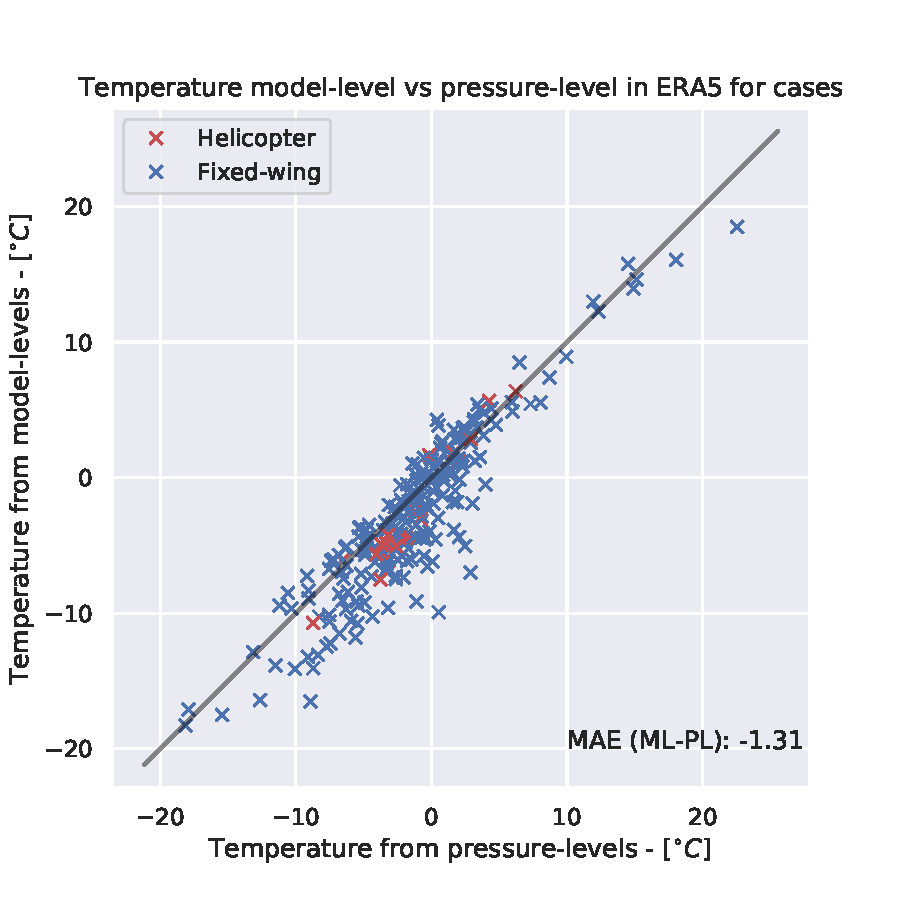
\includegraphics[width=\textwidth]{Figures/mlvspl.pdf}
    \caption{Scatter plot between model-level and pressure-level interpolation of temperature from ERA5, also printed on the figure: Mean Absolute Difference (MAD), showing model-level interpolation averagely colder than pressure level interpolation with $1.31^{\circ}$ Celsius.}
    \label{fig:mlvspltemp}
    \end{subfigure}
    \hfill
    \begin{subfigure}[h]{0.45\textwidth}
    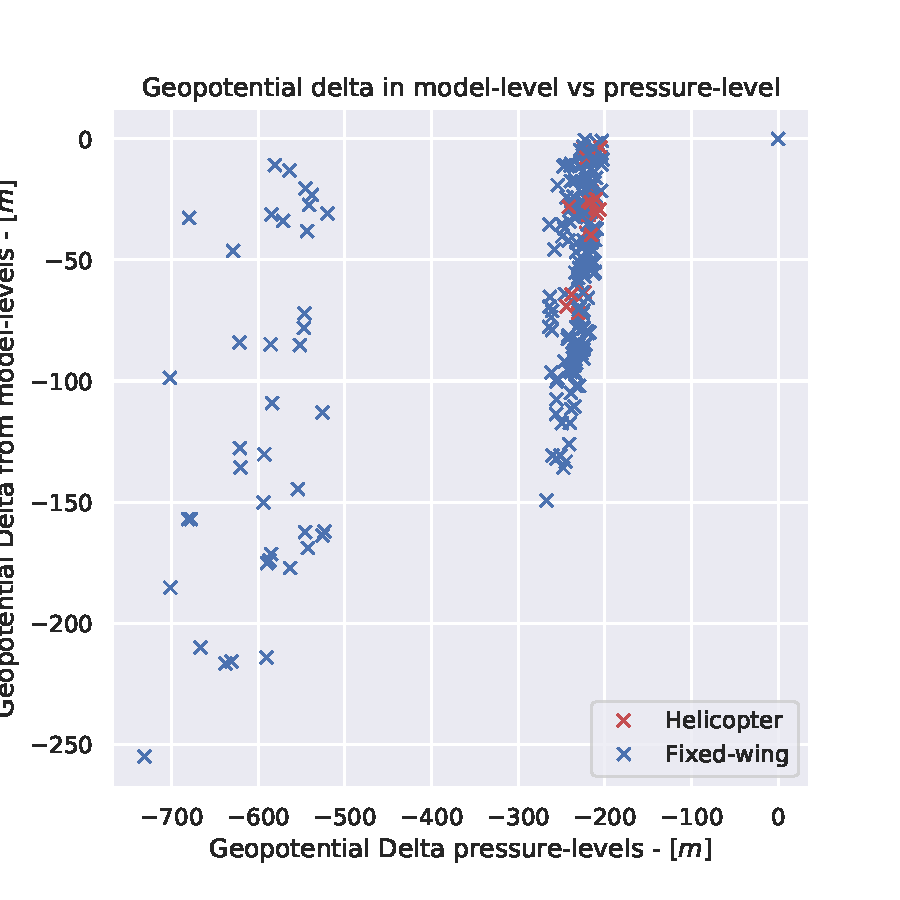
\includegraphics[width=\textwidth]{Figures/geopot.pdf}
    \caption{Scatter plot between model level and pressure level interpolation of geopotential height from ERA5.}
    \label{fig:mlvsplgeopot}
    \end{subfigure}
    \caption{Difference between model level and pressure level interpolations for a) Temperature and b) geopotential height. The temperature is found by geopotential height as discussed in Section \ref{sec:interpolation}, such that these variables are not independent.}
    \label{fig:mlvspl}
\end{figure}

\begin{figure}
    \centering
    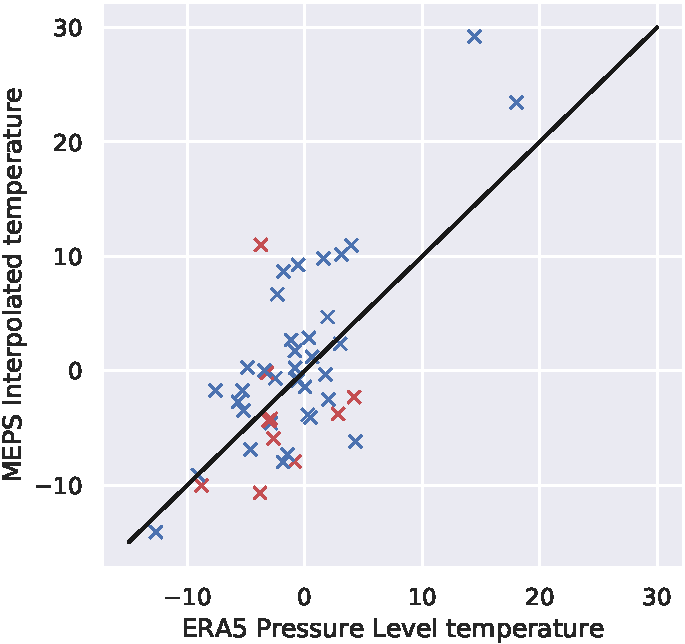
\includegraphics[width=.5\textwidth]{Figures/T750MEPSera5diff.pdf}
    \caption{Difference of ERA5 and MEPS temperatures using pressure level interpolation to case height.}
    \label{fig:eramepsdiff}
\end{figure}

\subsection{Loss in data due to archiving}
Due to the Meteorological Institute reducing their available archived model data, the vertical velocity parameter was not available for cases before October 2018. To perform the decomposition analysis, the vertical velocity sub-index was determined from its relation to \acrshort{hti}:

\[\frac{\text{Vertical Wind}}{4} = \text{HTI} - (\frac{\text{Temperature}}{4} + \frac{\text{Precipitation}}{4} +\frac{\text{Cloud}}{4}) \] 
Thus the \acrshort{hti} was needed to calculate the vertical velocity, and as such the cases where \acrshort{hti} was set to zero by the land-sea mask, the vertical velocity index was not retrievable. 